\chapter{敏捷开发流程}\label{chap:06-agility}

\section{整体测试思路}\label{sec:06-agility-001}

在软件的敏捷开发中，测试是确保软件质量的重要环节之一。对于硬件的开发来说，测试甚至更加重要，因为测试的难度更大。处理器的测试通常是在运行程序的过程中发现潜在的bug，并确保处理器在各种情况下都能正常运行。在处理器的开发过程中，针对不同的开发阶段，需要进行不同层次的测试。在开发初期，需要进行单元测试，以验证处理器的各个单元模块是否按照设计规格正确工作。随着不断迭代，还要进行回归测试和集成测试，以确保新的修改不会影响到原有功能，并且不同部件能够正确地集成在一起。由于程序的复杂性和多样性，bug往往会被隐藏在不同的场景中。因此，为了尽可能地发现潜在的问题，测试需要覆盖尽量多的程序类型，包括各种操作系统、应用程序以及特定场景下的测试用例。

因此，在硬件的敏捷开发环境下，我们需要一套更加成熟的测试方法，以在开发的各个阶段，对处理器进行不同维度的测试。测试还需要保持高度自动化，以提高测试效率，保证项目的敏捷迭代。本文将对硬件的敏捷开发方法进行概述，并介绍Chisel、DiffTest、AM、SoC集成等技术。

\section{AM}\label{sec:06-agility-002}

\subsection{AM简介}\label{sec:06-agility-003}

AM，即Abstract Machine，是由南京大学开发的一套裸机程序运行环境，其是计算机硬件最小、模块化、独立于机器的抽象层，旨在便捷地创建 LA32R 架构的裸机 C 程序及汇编程序，与指令集架构、操作系统、应用解耦。AM包含如下部分：

\begin{enumerate}
\def\labelenumi{\arabic{enumi}.}
\item
  图灵机（TRM）：物理内存和直接执行；
\item
  I/O扩展（IOE）：输入和输出设备的基本模型；
\item
  上下文扩展（CTE）：中断/异常和处理器上下文管理；
\item
  虚拟内存扩展（VME）：虚拟内存和保护；
\item
  多处理器扩展（MPE）：多处理器支持。
\end{enumerate}

我们知道，应用程序的运行都需要运行时环境的支持，而只进行纯粹计算任务的程序在TRM上就可以运行，它只需要：

\begin{enumerate}
\def\labelenumi{\arabic{enumi}.}
\item
  把程序放在正确的内存位置；
\item
  让PC指向第一条指令；
\item
  计算机自动执行程序。
\end{enumerate}

\subsection{AM配置方法}\label{sec:06-agility-004}

通过如下命令克隆仓库

% 代码语言：BookShell
\begin{CodeBlock}[language=BookShell]
$ git clone git@github.com:BUAA-CI-LAB/am.git
\end{CodeBlock}

可以看到，AM的目录结构如下：

\begin{itemize}
\tightlist
\item
  \texttt{am/}：AM头文件、每个体系结构分别实现的AM代码
\item
  \texttt{apps/}：一些 benchmark，如 coremark，dhrystone，linux
\item
  \texttt{tests/}: 用来测试 CPU/SoC 实现的测试程序
\end{itemize}

为了编译AM，首先需要设置环境变量。将环境变量 \texttt{AM\_HOME} 设置为 \textbf{am 项目的根目录的绝对路径}，如 \texttt{/home/am}。然后，设置 la32r 编译器与库的环境变量：将 \texttt{loongarch32r-linux-gnusf-2022-05-20} 与 \texttt{system\_newlib} 放在一个文件夹 \texttt{la32r-toolchains} 下，并将 \texttt{\$LA32RTC\_HOME} 环境变量设置为 \texttt{la32r-toolchains} 目录。

% 代码语言：BookText
\begin{CodeBlock}[language=BookText]
├── la32r-toolchains
│   ├── loongarch32r-linux-gnusf-2022-05-20
│   └── system_newlib
\end{CodeBlock}

编译时，首先确保环境变量是否正确设置，然后执行\texttt{make\ ARCH=体系结构-平台}编译。例如\texttt{make\ ARCH=la32r-eula} 编译生成可在 chiplab 及 DiffTest 仿真环境中运行的裸机程序。

\begin{itemize}
\tightlist
\item
  注意：在 \texttt{\$AM\_HOME} 下 \texttt{make} 只会生成 am 的 archive 文件，在 \texttt{tests} 或 \texttt{apps} 文件夹中 \texttt{make} 才会生成对应程序的 elf，bin 及反汇编文件。
\end{itemize}

\subsection{AM编写测试}\label{sec:06-agility-005}

事实上，AM中的所有测试都会共用 \texttt{ARCH} 指定的编译命令，链接脚本及初始化代码。以 \texttt{ARCH=la32r-eula} 为例，cpu 复位后指令流为：

% 代码语言：BookText
\begin{CodeBlock}[language=BookText]
am/src/eula/isa/la32r/boot/start.S        // 初始化栈指针
am/src/eula/isa/la32r/trm.c : _trm_init   // 初始化外设，初始化缓存，建立地址空间映射等
执行对应程序 main 函数
返回 _trm_init 执行 halt 函数结束仿真
\end{CodeBlock}

\begin{itemize}
\tightlist
\item
  目前在 \texttt{halt} 函数中尝试使用 \texttt{syscall\ 0x11} 指令结束程序运行。运行 AM 程序的目标平台应当支持此种方法（la32r-nemu 支持，因此使用 la32r-nemu 协同仿真的 DiffTest 框架及 chiplab 框架均支持此方法）。
\end{itemize}

如果需要编写单文件测试程序，Makefile 编写及文件夹结构请参考 \texttt{tests/cputest}

如果需要编写多文件测试程序，注意程序用C/C++语言编写，除AM之外无法调用其他库函数（但可以引用\texttt{stdarg.h}, \texttt{limits.h}等包含体系结构相关数据定义的头文件）。

为此你需要在应用程序项目的根目录添加一个Makefile（以 \texttt{apps/coremark} 为例）：

% 代码语言：BookMake
\begin{CodeBlock}[language=BookMake]
NAME = coremark
SRCS = $(shell find -L ./src/ -name "*.c")
include $(AM_HOME)/Makefile.app
\end{CodeBlock}

一些注意事项：

\begin{itemize}
\item
  \texttt{NAME}定义了应用的名字。编译后会在\texttt{build/}目录里出现以此命名的应用程序
\item
  \texttt{SRCS}指定了编译应用所需的源文件。可以放在应用目录中的任意位置
\item
  应用目录下的\texttt{include/}目录会被添加到编译的\texttt{-I}选项中
\end{itemize}

\section{Chisel}\label{sec:06-agility-006}

\subsection{Scala简介}\label{sec:06-agility-007}

Scala是一种多范式编程语言，它结合了面向对象编程和函数式编程的特性，具有强大的表达能力和灵活的语法。相较Java，其简化了Java大部分冗余的语法，并共享相同的底层类型和运行时。而Scala可以使用任何现成的Java库，包括Java标准库，这意味着几乎任何Java程序都可以在Scala中以相同的方式工作。Scala的名字源于Scalable Language，即可拓展语言，Scala 不仅可以根据硬件资源和负载要求进行扩展，还可以根据程序员的技能水平进行扩展。

在Scala中，class和object的概念尤为重要，class是创建object的蓝图，定义一个class后，我们就可以从该类创建新的object。

例如，你可以通过如下的方式定义class和object：

% 代码语言：BookScala
\begin{CodeBlock}[language=BookScala]
// 定义一个抽象类Animal
abstract class Animal(var name: String) {
  def sound(): String // 抽象方法，子类需要实现
}

// 定义一个Dog类，继承自Animal
class Dog(name: String, var breed: String) extends Animal(name) {
  override def sound(): String = "Woof" // 实现抽象方法，返回狗的叫声
}

// 定义一个Cat类，继承自Animal
class Cat(name: String, var color: String) extends Animal(name) {
  override def sound(): String = "Meow" // 实现抽象方法，返回猫的叫声
}

// 定义一个Companion Object，包含apply方法
object Animal {
  // apply方法用于创建Animal对象
  def apply(name: String, animalType: String): Animal = {
    animalType match {
      case "dog" => new Dog(name, "Unknown")
      case "cat" => new Cat(name, "Unknown")
      case _ => throw new IllegalArgumentException("Unknown animal type!")
    }
  }
}

object Main extends App {
  // 使用apply方法创建Dog和Cat对象
  val dog = Animal("Buddy", "dog")
  val cat = Animal("Whiskers", "cat")

  // 打印狗和猫的信息
  println(s"${dog.name} is a ${dog.getClass.getSimpleName}, breed: ${dog.asInstanceOf[Dog].breed}, sound: ${dog.sound()}")
  println(s"${cat.name} is a ${cat.getClass.getSimpleName}, color: ${cat.asInstanceOf[Cat].color}, sound: ${cat.sound()}")
}
\end{CodeBlock}

代码定义了一个抽象类Animal，它有一个抽象方法sound()，代表动物的叫声。然后定义了两个具体的动物类，Dog和Cat，它们都继承自Animal类，并实现了sound()方法。

在Scala中，伴生对象 (object) 是与类同名的对象，它与类在同一个文件中定义，并且可以访问类的私有成员。在上面的代码中，Animal类的伴生对象object Animal扮演了一个工厂的角色，它定义了一个apply方法，根据传入的参数创建不同类型的对象。apply方法是一个特殊的方法，它允许我们像调用函数一样创建对象，而不需要使用new关键字。比如，我们可以使用Animal(``Buddy'', ``dog'')来创建一个名为Buddy的狗对象，scala将自动调用 apply 方法。

在Scala中，我们将程序的入口点定义在一个对象中，并且该对象可以扩展自App trait。App trait提供了一个方便的方式来编写简单的应用程序，它自动为我们处理了main方法的实现。在本段代码中，Main对象继承了App trait，程序将从此开始运行。

\subsection{Chisel库简介}\label{sec:06-agility-008}

与软件开发相比，硬件开发受到开发工具的影响更为显著。硬件敏捷开发宣言的第三项原则强调了优化工具和生成器的重要性，而不是单纯优化个别实例。

在这个背景下，USB团队开发了一种新型的硬件构建语言------Chisel。Chisel基于Scala开发，具备高度的复用性和可扩展性，并由UCB团队在开发RocketChip的同时进行了开发。通过在Scala中定义类和对象，Chisel赋予了硬件电路以编程语义。使用者可以通过Chisel库中的原语来描述电路，然后将代码转化为Verilog代码，以供现有的EDA工具使用。

Chisel采用了面向对象的设计模式，将硬件描述抽象为Scala中的类和对象。这使得Chisel代码具有良好的组织结构和模块化，易于理解和维护。同时，Chisel还借鉴了Scala的函数式编程特性，如高阶函数、不可变性和函数组合等。这使得Chisel代码更加简洁、灵活和易于并行化，同时也为硬件验证和测试提供了更好的支持。因此，学习Scala语言对于理解和使用Chisel是至关重要的。Scala语言具有丰富的语法和功能，包括面向对象编程、函数式编程、模式匹配、类型推断等。这些功能不仅可以帮助我们更好地理解Chisel代码，还可以提高我们的编程技能和抽象能力。此外，Scala语言还具有强大的类型系统和丰富的标准库，可以为我们提供更多的工具和资源来编写高效、优雅的Chisel代码。

\subsection{Chisel环境的配置方法}\label{sec:06-agility-009}

\begin{enumerate}
\def\labelenumi{\arabic{enumi}.}
\tightlist
\item
  安装Java Development Kit (JDK)：Scala是基于Java平台的，因此首先需要安装JDK。可以从Oracle官网或者OpenJDK项目获取JDK的安装包。安装完成后，需要设置JAVA\_HOME环境变量，并且将Java的bin目录添加到系统的PATH环境变量中。
\item
  下载Scala安装包：访问Scala官方网站（\url{https://www.scala-lang.org/}），在下载页面选择适合操作系统的Scala版本。
\item
  配置环境变量：安装完成后，设置SCALA\_HOME环境变量，指向你安装Scala的目录。然后将Scala的bin目录添加到系统的PATH环境变量中，这样你就可以在命令行中直接运行Scala解释器和编译器。
\item
  验证安装：输入命令\texttt{scala\ -version}和\texttt{scalac\ -version}分别验证Scala解释器和编译器的版本。如果显示了相应的版本信息，则说明Scala环境已成功配置。
\item
  构建工具：Scala通常与一些流行的构建工具一起使用，如sbt（Scala Build Tool）和mill。\%TODO
\item
  获取Chisel源码：通过Git工具将Chisel克隆到本地:`git clone \url{https://github.com/freechipsproject/chisel3.git}
\item
  构建Chisel：进入Chisel源码目录，执行以下命令构建Chisel：
\end{enumerate}

% 代码语言：BookShell
\begin{CodeBlock}[language=BookShell]
cd chisel3
sbt compile
\end{CodeBlock}

\begin{enumerate}
\def\labelenumi{\arabic{enumi}.}
\setcounter{enumi}{7}
\tightlist
\item
  验证安装：构建完成后，可以在Chisel源码目录下执行以下命令来运行Chisel的测试：\texttt{sbt\ test}
\end{enumerate}

\subsection{Chisel的使用技巧}\label{sec:06-agility-010}

\begin{enumerate}
\def\labelenumi{\arabic{enumi}.}
\tightlist
\item
  Chisel可以支持参数化的硬件生成，例如：
\end{enumerate}

% 代码语言：BookScala
\begin{CodeBlock}[language=BookScala]
object TopMain extends App {
  def parseArgs(info: String, args: Array[String]): String = {
    var target = ""
    for (arg <- args) { if (arg.startsWith(info + "=") == true) { target = arg } }
    require(target != "")
    target.substring(info.length()+1)
  }
  val board = parseArgs("BOARD", args)
  val core = parseArgs("CORE", args)
  
  val s = (board match {
    case "sim"    => Nil
    case "perftest" => PerfTestSettings()
    case "chiplab" => Nil
    case "megasoc" => Nil
  } ) ++ ( core match {
    case "inorder"  => InOrderSettings()
    case "ooo"  => OOOSettings()
  } )
  s.foreach{Settings.settings += _} // add and overwrite DefaultSettings
  println("====== Settings = (" + board + ", " +  core + ") ======")
  Settings.settings.toList.sortBy(_._1)(Ordering.String).foreach {
    case (f, v: Long) =>
      println(f + " = 0x" + v.toHexString)
    case (f, v) =>
      println(f + " = " + v)
  }
  if (board == "sim") {
    (new ChiselStage).execute(args, Seq(
      ChiselGeneratorAnnotation(() => new SimTop))
    )
  } else if (board == "perftest" || board == "megasoc") {
    (new ChiselStage).execute(args, Seq(
      ChiselGeneratorAnnotation(() => new Top))
    )
  } else if (board == "chiplab") {
    (new ChiselStage).execute(args, Seq(
      ChiselGeneratorAnnotation(() => new ChiplabTop))
    )
  } else {
    println("board is unavailable")
    assert(false)
  }
}
\end{CodeBlock}

这段代码实现了Chisel代码的参数化，即根据命令行参数来配置不同的硬件设计选项。parseArgs函数用于解析命令行参数。它接受一个描述信息字符串和一个参数数组，并返回与该描述信息对应的参数值。例如，parseArgs(``BOARD'', args)将返回命令行参数中以''BOARD=``开头的参数值，以确定该处理器运行在什么样的板卡上。根据解析得到的board和core参数值，构造了一个设置列表s。该列表根据不同的board和core参数值，选择性地包含了特定的设置项，并将构造的设置列表s添加到默认设置中。最后，根据board参数的值选择要生成的顶层模块，并使用Chisel的ChiselStage执行代码生成verilog。根据不同的board参数值，选择生成不同的顶层模块，如SimTop、Top或ChiplabTop等。通过这种方式，可以在命令行中灵活地指定不同的参数值，从而生成不同配置的硬件设计。这种参数化设计的好处在于，可以方便地进行定制和调整，使得硬件设计更加灵活和易于维护。

\begin{enumerate}
\def\labelenumi{\arabic{enumi}.}
\setcounter{enumi}{1}
\tightlist
\item
  Chisel中的BlackBox特性，可以支持实例化外部定义的模块，此特性对于使用Chisel中未定义的IP较为有用。首先BlackBox模块将在生成的Verilog中实例化，但不会生成任何代码来定义模块的行为。与Module不同，BlackBox没有隐式时钟和复位。BlackBox的时钟和复位端口必须明确声明并连接到输入信号。IO Bundle中声明的端口将使用请求的名称生成（即没有前面的 io\_）。
\end{enumerate}

通过以下方式，我们可以定义一个名为Core的BlackBox

% 代码语言：BookScala
\begin{CodeBlock}[language=BookScala]
class Core extends BlackBox {
  override val desiredName = "mycpu_mega_top"
  val io = IO(new Bundle {
    val out = new AXI4
    val ext_int = Input(UInt(8.W))
    val clock = Input(Clock())
    val reset = Input(Bool())
  }).suggestName("io")

  forceName(io.out.ar.bits.id, "arid")
  forceName(io.out.ar.bits.addr, "araddr")
  forceName(io.out.ar.bits.len, "arlen")
  forceName(io.out.ar.bits.size, "arsize")
  forceName(io.out.ar.bits.burst, "arburst")
  forceName(io.out.ar.bits.lock, "arlock")
  forceName(io.out.ar.bits.cache, "arcache")
  forceName(io.out.ar.bits.prot, "arprot")
  forceName(io.out.ar.bits.qos, "arqos")
  forceName(io.out.ar.bits.user, "aruser")
  forceName(io.out.ar.valid, "arvalid")
  forceName(io.out.ar.ready, "arready")

  forceName(io.out.r.bits.id, "rid")
  forceName(io.out.r.bits.data, "rdata")
  forceName(io.out.r.bits.resp, "rresp")
  forceName(io.out.r.bits.last, "rlast")
  forceName(io.out.r.bits.user, "ruser")
  forceName(io.out.r.valid, "rvalid")
  forceName(io.out.r.ready, "rready")

  forceName(io.out.aw.bits.id, "awid")
  forceName(io.out.aw.bits.addr, "awaddr")
  forceName(io.out.aw.bits.len, "awlen")
  forceName(io.out.aw.bits.size, "awsize")
  forceName(io.out.aw.bits.burst, "awburst")
  forceName(io.out.aw.bits.lock, "awlock")
  forceName(io.out.aw.bits.cache, "awcache")
  forceName(io.out.aw.bits.prot, "awprot")
  forceName(io.out.aw.bits.qos, "awqos")
  forceName(io.out.aw.bits.user, "awuser")
  forceName(io.out.aw.valid, "awvalid")
  forceName(io.out.aw.ready, "awready")

  // forceName(io.out.w.bits.id, "wid")
  forceName(io.out.w.bits.data, "wdata")
  forceName(io.out.w.bits.strb, "wstrb")
  forceName(io.out.w.bits.last, "wlast")
  forceName(io.out.w.valid, "wvalid")
  forceName(io.out.w.ready, "wready")

  forceName(io.out.b.bits.id, "bid")
  forceName(io.out.b.bits.resp, "bresp")
  forceName(io.out.b.bits.user, "buser")
  forceName(io.out.b.valid, "bvalid")
  forceName(io.out.b.ready, "bready")
}
\end{CodeBlock}

该段代码声明了一个处理器的BlackBox，在生成Verilog时，该BlackBox实例化时的模块名会被定义为mycpu\_mega\_top，而out端口代表一系列AXI4相关的接口，其接口可以通过forceName特性进行强制命名。

\begin{enumerate}
\def\labelenumi{\arabic{enumi}.}
\setcounter{enumi}{2}
\tightlist
\item
  接口复用
\end{enumerate}

如上述代码所示，我们对AXI4的接口类进行了复用，实际其定义如下：

% 代码语言：BookScala
\begin{CodeBlock}[language=BookScala]
class AXI4(val dataBits: Int = AXI4Parameters.dataBits, val idBits: Int = AXI4Parameters.idBits) extends AXI4Lite {
  override val aw = Decoupled(new AXI4BundleA(idBits))
  override val w  = Decoupled(new AXI4BundleW(dataBits))
  override val b  = Flipped(Decoupled(new AXI4BundleB(idBits)))
  override val ar = Decoupled(new AXI4BundleA(idBits))
  override val r  = Flipped(Decoupled(new AXI4BundleR(dataBits, idBits)))
}
\end{CodeBlock}

注意到，AXI4接口类继承了AXI4Lite接口类，AXI4Lite接口类定义如下：

% 代码语言：BookScala
\begin{CodeBlock}[language=BookScala]
class AXI4Lite extends Bundle {
  val aw = Decoupled(new AXI4LiteBundleA)
  val w  = Decoupled(new AXI4LiteBundleW)
  val b  = Flipped(Decoupled(new AXI4LiteBundleB))
  val ar = Decoupled(new AXI4LiteBundleA)
  val r  = Flipped(Decoupled(new AXI4LiteBundleR))
}
\end{CodeBlock}

可以发现，其中也对AXI4LiteBundleA、new AXI4LiteBundleW、new AXI4LiteBundleB、AXI4LiteBundleR这类接口进一步进行了复用。

\begin{enumerate}
\def\labelenumi{\arabic{enumi}.}
\setcounter{enumi}{3}
\tightlist
\item
  Decoupled和Flipped
\end{enumerate}

上述代码中使用到了Decoupled和Flipped特性，其含义为将接口包装一层valid和ready握手信号，Decoupled默认方向为输出，如果需要输入，可以在Decoupled外再套一层Flipped，正如前面代码所展示的。

6.3.3 ChiselTest：前端设计时的单元测试和回归测试

\section{verilator}\label{sec:06-agility-011}

\subsection{verilator仿真流程简介}\label{sec:06-agility-012}

Verilator 是一个开源的硬件描述语言（如 Verilog 和 SystemVerilog）仿真工具，它能够将硬件描述代码转换为 C++ 或 SystemC 代码，然后进行编译，并通过 C++ 编译器或 SystemC 仿真器来执行，适合基于敏捷开发流程的工程实践。

Verilator 首先会读取 Verilog 或 SystemVerilog 代码，并解析其语法和语义，并转换为等效的 C++ 代码。这个过程包括了将 Verilog 或 SystemVerilog 的语法结构映射到 C++ 的数据结构和函数调用。例如，Verilog 中的模块会被转换为 C++ 一个类，模块的端口会被转换为类的成员变量，模块的行为逻辑会被转换为类的成员函数。生成的 C++ 代码会包含对应的硬件模块和逻辑。同时，Verilator 也会添加一些额外的代码，用于管理仿真的执行流程和状态，包括时钟、事件触发、信号更新等，以保证仿真的正确执行。最后，生成的 C++ 代码会由 clang 编译成可执行文件，执行该文件的过程就是对 Verilog 代码进行仿真的过程。

下面以一个时序逻辑电路为例，讨论verilator仿真的原理。

% 代码语言：BookVerilog
\begin{CodeBlock}[language=BookVerilog]
// detect.v

module detect (
    input clk,
    input data_in,
    input reset,
    output reg out
);

reg [1:0] pattern;

always @(posedge clk or posedge reset) begin
    if (reset) begin
        pattern <= 2'b00;
        out <= 0;
    end else begin
        pattern <= {pattern[0], data_in};
        out <= (pattern == 2'b01);
    end
end

endmodule
\end{CodeBlock}

使用verilator进行编译 \texttt{verilator\ -\/-cc\ detect.v，之后可在}obj\_dir` 中找到生成的 C++ 代码文件。

% 代码语言：BookCpp
\begin{CodeBlock}[language=BookCpp]
// Vdetect.h
// This class is the main interface to the Verilated model
class Vdetect VL_NOT_FINAL {
  private:
    // Symbol table holding complete model state (owned by this class)
    Vdetect__Syms* const vlSymsp;

  public:

    // PORTS
    // The application code writes and reads these signals to
    // propagate new values into/out from the Verilated model.
    VL_IN8(&clk,0,0);
    VL_IN8(&reset,0,0);
    VL_IN8(&data_in,0,0);
    VL_OUT8(&out,0,0);

    // CELLS
    // Public to allow access to /* verilator public */ items.
    // Otherwise the application code can consider these internals.

    // Root instance pointer to allow access to model internals,
    // including inlined /* verilator public_flat_* */ items.
    Vdetect___024root* const rootp;

    // CONSTRUCTORS
    /// Construct the model; called by application code
    /// If contextp is null, then the model will use the default global context
    /// If name is "", then makes a wrapper with a
    /// single model invisible with respect to DPI scope names.
    explicit Vdetect(VerilatedContext* contextp, const char* name = "TOP");
    explicit Vdetect(const char* name = "TOP");
    /// Destroy the model; called (often implicitly) by application code
    virtual ~Vdetect();
  private:
    VL_UNCOPYABLE(Vdetect);  ///< Copying not allowed

  public:
    // API METHODS
    /// Evaluate the model.  Application must call when inputs change.
    void eval() { eval_step(); }
    /// Evaluate when calling multiple units/models per time step.
    void eval_step();
    /// Evaluate at end of a timestep for tracing, when using eval_step().
    /// Application must call after all eval() and before time changes.
    void eval_end_step() {}
    /// Simulation complete, run final blocks.  Application must call on completion.
    void final();
    /// Return current simulation context for this model.
    /// Used to get to e.g. simulation time via contextp()->time()
    VerilatedContext* contextp() const;
    /// Retrieve name of this model instance (as passed to constructor).
    const char* name() const;
} VL_ATTR_ALIGNED(VL_CACHE_LINE_BYTES);
\end{CodeBlock}

其中的注释由 verilator 自动生成。可以看出，verilog代码中的 \texttt{detect} 模块被翻译为乐一个 C++ 类。每个输入输出端口被转换为一个成员，例如时钟输被翻译为 \texttt{VL\_IN8(\&clk,0,0);}。在每个模块中调用 \texttt{eval()} 方法，可完成一个周期内对模块行为，也包括输出信号数值的更新。\texttt{final()} 用于在结束仿真时释放资源。\texttt{contextp()} 和 \texttt{name()} 用于获取模型的当前仿真上下文和模型的实例名称。

% 代码语言：BookCpp
\begin{CodeBlock}[language=BookCpp]
// Vdetect___[some number].cpp
VL_INLINE_OPT void Vdetect___024root___sequent__TOP__0(Vdetect___024root* vlSelf) {
	// Init ...
    // Body
    __Vdly__detect__DOT__pattern = vlSelf->detect__DOT__pattern;
    if (vlSelf->reset) {
        __Vdly__detect__DOT__pattern = 0U;
        vlSelf->out = 0U;
    } else {
        __Vdly__detect__DOT__pattern = ((2U & ((IData)(vlSelf->detect__DOT__pattern) 
                                               << 1U)) 
                                        | (IData)(vlSelf->data_in));
        vlSelf->out = (1U == (IData)(vlSelf->detect__DOT__pattern));
    }
    vlSelf->detect__DOT__pattern = __Vdly__detect__DOT__pattern;
}
void Vdetect___024root___eval(Vdetect___024root* vlSelf) {
	// Init ...
	// Body
    if ((((IData)(vlSelf->clk) & (~ (IData)(vlSelf->__Vclklast__TOP__clk))) 
         | ((IData)(vlSelf->reset) & (~ (IData)(vlSelf->__Vclklast__TOP__reset))))) {
        Vdetect___024root___sequent__TOP__0(vlSelf);
    }
    // Final
    vlSelf->__Vclklast__TOP__clk = vlSelf->clk;
    vlSelf->__Vclklast__TOP__reset = vlSelf->reset;
}

// Vdetect.cpp
void Vdetect::eval_step() {
    VL_DEBUG_IF(VL_DBG_MSGF("+++++TOP Evaluate Vdetect::eval_step\n"); );
#ifdef VL_DEBUG
    // Debug assertions
    Vdetect___024root___eval_debug_assertions(&(vlSymsp->TOP));
#endif  // VL_DEBUG
    // Initialize
    if (VL_UNLIKELY(!vlSymsp->__Vm_didInit)) _eval_initial_loop(vlSymsp);
    // Evaluate till stable
    do {
        VL_DEBUG_IF(VL_DBG_MSGF("+ Clock loop\n"););
        Vdetect___024root___eval(&(vlSymsp->TOP));
    } while (0);
    // Evaluate cleanup
}

\end{CodeBlock}

代码中的 \texttt{Vdetect\_\_\_024root\_\_\_sequent\_\_TOP\_\_0} 函数是 Verilog 模块中 always 块的仿真函数。它包含了 Verilog 模块的时序逻辑，即在时钟上升沿或复位信号上升沿时的行为。其中，\texttt{\_\_Vdly\_\_detect\_\_DOT\_\_pattern} 对应于 Verilog 中的寄存器 \texttt{pattern}，用于存储模块的状态。在每个时钟周期中，该函数会根据输入信号的变化更新模块的状态，并计算输出信号的值。\texttt{Vdetect\_\_\_024root\_\_\_eval} 函数是整个模块的评估函数，用于驱动仿真过程。它检测时钟信号和复位信号的变化，并在调用 \texttt{Vdetect\_\_\_024root\_\_\_sequent\_\_TOP\_\_0} 函数执行仿真逻辑，确保模块的输出在每个时钟周期内得到正确更新。\texttt{void\ Vdetect::eval\_step()} 函数用于执行仿真过程，它首先调用 \texttt{Vdetect\_\_\_024root\_\_\_eval} 函数执行评估操作，然后重复执行。

常见的仿真方法是基于事件驱动的，仿真器跟踪每个信号的状态变化，并在信号发生变化时触发相应的事件。仿真器通常会维护一个事件队列，记录下一次事件发生的时间以及需要执行的操作。当仿真器推进时间时，它会检查事件队列，找到下一个要发生的事件，并执行相应的操作，例如更新信号的值、调用触发器的行为等。这种方法只需处理信号的变化，提高了仿真效率和准确率，能够有效处理大型复杂的电路。

而Verilator 采用的则是基于编译的仿真方法，将硬件描述语言转换为等效的 C++ 代码，并在C++的执行过程中完成仿真。这种方法通常比传统的基于事件驱动的仿真器更快，因为它避免了在运行时解释硬件描述语言的开销。

敏捷开发的过程强调快速迭代，因此仿真器的仿真速度是十分重要的。使用Verilator进行的仿真可以使开发者获得即时的反馈，快速验证设计的正确性，有助于在迭代过程中及早发现和解决问题。

Verilator的第二个优势是可以简单地与 C/C++ 代码进行集成。由于 verilator 本来就要将待测模型翻译为 C++，因此在仿真过程中调用 C/C++ 代码变得十分自然。Verilator 可以集成软件编写的测试框架、性能分析工具等，使用 verilator 编译后即可将软件代码和硬件代码编译到一个可执行文件中，在整个开发流程中使用一致的仿真环境和工具链。

\subsection{verilator仿真的优缺点}\label{sec:06-agility-013}

Verilator工具开源，支持自主定制，且仿真操作简单，速度快，但其问题在于仅能仿真二态，难以通过Verilator仿真检测不定态和高阻态。因此，对于仿真需精度需求更高的测试，可以采用Synopsys公司推出的商业Verilog仿真器VCS，即 Verilog Compiler Simulator。VCS具有高效的仿真引擎和优化的仿真算法，可以处理大规模的设计，并获得较快的仿真速度，提供了对Verilog和SystemVerilog的全面支持。但是，VCS 需要购买许可证才能使用，成本较高，并且安装和学习成本较高。

\section{DiffTest 差分测试}\label{sec:06-agility-014}

\subsection{差分测试简介}\label{sec:06-agility-015}

国科大团队在 2022 年提出了一种新的测试方法，名为差分测试方法。该团队注意到，使用同一个指令集架构的处理器芯片，虽然可能有着不同的微结构设计，但却一定都符合指令集架构的要求。因此，该团队将验证框架和微结构设计进行解耦，开发了名为DiffTest的差分测试框架，并使用该框架及其他测试工具成功开发了一款高性能的RISC-V处理器。该验证方法只对处理器的体系结构状态合法性进行验证，而不验证完整的微结构状态合法性。即，该框架只在检测到待测模块体系结构状态不符合指令集架构规范的证据时，才会报错。

\subsection{体系结构模拟器}\label{sec:06-agility-016}

NEMU是由南京大学团队开发的体系结构模拟器，其可以模拟一个RISC-V/LA32R单周期处理器，在程序运行时以动态链接库的形式作为DiffTest差分测试的基准。原DiffTest框架中的refproxy类对调用动态链接库中函数的过程进行了封装，用于获取NEMU运行时的状态。

\subsection{接口与微结构状态}\label{sec:06-agility-017}

以下将通过演示在DiffTest中添加TLB表项比对功能进一步介绍DiffTest的接入与使用。以TLB重填为例，指令集架构只规定TLB重填时可根据某种规则选择一个表项位置进行重填，但没有规定选择重填位置的具体规则。使用者希望可以检测参考模型和待测处理器的TLB表项内容是否一致，从而验证TLB模块开发的正确性，但参考模型无法感知待测处理器内部实现的重填规则。因此，我们要求待测处理器进行TLB重填时，将重填的表项下标传递给DiffTest框架，DiffTest框架将该信息传递给参考模型，使参考模型内部也对相应的 TLB 表项进行重填。

LA32R 指令集采用双页结构，一个 TLB表项包含hi、lo0、lo1三部分，其中hi中储存虚拟地址，lo0和lo1部分分别对应该表项对应的奇偶两个物理页地址。首先需要在 DiffTest 框架中 Chisel 部分增加监视器，将 TLB 重填事件和 TLB 表项传递给该框架。

% 代码语言：BookScala
\begin{CodeBlock}[language=BookScala]
class DiffLa32rTlbFillIndexSetIO extends DifftestBundle {
  val valid = Input(Bool())
  val index = Input(UInt(8.W))
}

class DiffLa32rTlbEntryIO extends DifftestBundle with DifftestWithIndex {
  val entryhi = Input(UInt(64.W))
  val entrylo0 = Input(UInt(32.W))
  val entrylo1 = Input(UInt(32.W))
}
\end{CodeBlock}

然后，由于原先的NEMU模拟器不支持TLB表项的读取，因此需要对其进行调整。

在NEMU的LA32R目录下实现了isa\_tlbcpy\_to\_difftest函数，该函数向传入的TLB表项指针指向的地址中，写入当前NEMU内部的表项值。 之后，在cpu目录下对该函数进行了封装，得到difftest\_tlbcpy\_to\_difftest函数。

% 代码语言：BookCpp
\begin{CodeBlock}[language=BookCpp]
// isa/la32r/difftest/ref.c
void isa_tlbcpy_to_difftest(uint32_t index, void *dut) {
  struct tlb_struct* tlb_temp = (struct tlb_struct*) dut;
  tlb_temp->hi = tlb[index].hi;
  tlb_temp->lo[0] = tlb[index].lo[0];
  tlb_temp->lo[1] = tlb[index].lo[1];
}
// cpu/difftest/ref.c
void difftest_tlbcpy_to_difftest(uint32_t index, void *dut) {
  isa_tlbcpy_to_difftest(index, dut);
}
\end{CodeBlock}

DiffTest使用了posix标准库函数dlsym，其用于在动态链接库中查找符号并返回其地址。如下述代码所示，handle为已打开的NEMU动态链接库，通过调用dlsym函数查找名为difftest\_tlbcpy\_to\_difftest、difftest\_tlbcpy和difftest\_tlbfill\_index\_set的函数，并强制类型转换为函数指针形式，以供DiffTest内部直接使用。若动态链接库中没有找到相应名称的函数，则会使函数指针为null，因此在调用dlsym 后需要使用 check\_and\_assert 对其进行判断，在出现错误时及时报错，以增强代码的可维护性。

% 代码语言：BookCpp
\begin{CodeBlock}[language=BookCpp]
tlbcpy = (void (*)(uint32_t, void*))dlsym(handle, "difftest_tlbcpy_to_difftest");
check_and_assert(tlbcpy);
tlbcpy_to_nemu = (void (*)(uint32_t, void*))dlsym(handle, "difftest_tlbcpy");
check_and_assert(tlbcpy_to_nemu);
tlbfill_index_set = (void(*)(uint32_t))dlsym(handle,"difftest_tlbfill_index_set");
check_and_assert(tlbfill_index_set);
\end{CodeBlock}

至此，我们已经在DiffTest中得到了NEMU的TLB表项数据，下一步修改DiffTest::step函数，调整差分测试比对逻辑。为了向模拟器同步 TLB 重填下标，需要在 step 函数开始处检测处理器是否出发TLB重填事件，并将重填位置发送给模拟器。在模拟器执行指令后，从模拟器拷贝模拟器的所有 TLB 表项，并与待测模型的所有表项进行比对。

% 代码语言：BookCpp
\begin{CodeBlock}[language=BookCpp]
int Difftest::step() {
  // ...
  if (dut.la32r_tlbfill_idx_sync.valid) {
    proxy->tlbfill_index_set(dut.la32r_tlbfill_idx_sync.index);
  }
  // ...
  do_instr_commit();
  if (enable_tlb_diff && tlbmodify) {
    for (int i = 0; i < LA32R_TLB_ENTRY_NUM; i++) {
      proxy->tlbcpy(i, &(ref.la32r_tlb_entrys[i]));
    }
    bool consistent = !memcmp(
      dut.la32r_tlb_entrys, ref.la32r_tlb_entrys,
      sizeof(la32r_tlb_entry_t) * LA32R_TLB_ENTRY_NUM
    );
    if (!consistent) {
      display();
      return 1;
    }
  }
  // ...
  return 0;
}
\end{CodeBlock}

该段代码中，DiffTest 框架会在待测处理器出发 TLB 重填事件时，进入第一个条件分支内部，并使用已封装的 tlbfill\_index\_set 函数将待测处理器的重填位置传入模拟器，其中proxy是一个NEMU动态链接库封装后的指针。之后，该框架调用的do\_instr\_commit函数将控制模拟器执行一条指令。之后，该框架需要对模拟器和待测处理器的状态进行比对。

至此，我们便完成了DiffTest和NEMU的功能开发，最后只需要在处理器中实例化相应的DiffTest模块并进行连线。

% 代码语言：BookScala
\begin{CodeBlock}[language=BookScala]
val diffTlbFillIdxSync = Module(new DifftestLa32rTlbFillIndexSet)
diffTlbFillIdxSync.io.clock := clock
diffTlbFillIdxSync.io.coreid := 0.U
diffTlbFillIdxSync.io.valid := tlbModifyValid && tlbModifyOp === La32rCSROpType.tlbfill
diffTlbFillIdxSync.io.index := tlbFillIdx
    
val diffTlbEntry = Module(new DifftestLa32rTlbEntry)
diffTlbEntry.io.clock := clock
diffTlbEntry.io.index := i.U
diffTlbEntry.io.coreid := 0.U
diffTlbEntry.io.entryhi := tlbEntrys(i).tlbhi.asUInt()
diffTlbEntry.io.entrylo0 := tlbEntrys(i).tlblo0.asUInt()
diffTlbEntry.io.entrylo1 := tlbEntrys(i).tlblo1.asUInt()
\end{CodeBlock}

\section{SoC 验证}\label{sec:06-agility-018}

此部分结合具体内容介绍SoC的测试方法，要和《教学大纲》里SoC集成规范呼应，参考田学长毕业设计。（FPGA版本的SoC集成与验证）

\subsection{DPI-C 接口}\label{sec:06-agility-019}

SystemVerilog 直接编程接口 (DPI)基本上是SystemVerilog与外部编程语言（特别是C语言）之间的接口。它允许设计人员轻松地从SystemVerilog 调用 C 函数并导出 SystemVerilog 函数，以便可以从 C 调用它们。

DPI 具有很大的优势：它允许用户重用现有的 C 代码，并且不需要了解 Verilog 编程语言接口 (PLI) 或 Verilog 过程接口 (VPI) 接口。它还提供了一种调用部分（但不是全部）PLI 或 VPI 函数的替代（更简单）方法。 可以使用导入``DPI''声明从 SystemVerilog 调用用 C 实现的函数。我们将这些函数称为导入的任务和函数。所有导入的任务和函数都必须声明。在 SystemVerilog 中实现并在导出``DPI''声明中指定的函数和任务可以从 C 调用。我们将这些任务和函数称为导出的任务和函数。

DPI旨在在程序调用的软件级别上将 C语言与硬件描述语言相结合。在本芯片的仿真验证中，DPI-C 的用途是使 System Verilog 代码可以调用 C 语言编写的函数，进而能够在 C语言环境下使用操作系统的标准 API 进行通信。

这里给出了一个例子。一个名为 Bus 的模块包含两个函数：write，这是一个 SystemVerilog 函数，也导出到 C，以及一个名为 slave\_write 的函数，它从 C 导入。这两个函数都返回 void。 SystemVerilog：

% 代码语言：BookSystemVerilog
\begin{CodeBlock}[language=BookSystemVerilog]
module Bus(input In1, output Out1);
  import "DPI" function void slave_write(input int address,
                                         input int data);
  export "DPI" function write;  // Note – not a function prototype

  // This SystemVerilog function could be called from C
  function void write(int address, int data);
    // Call C function
    slave_write(address, data); // Arguments passed by copy
  endfunction
  ...
endmodule
\end{CodeBlock}

C:

% 代码语言：BookC
\begin{CodeBlock}[language=BookC]
#include "svdpi.h"
extern void write(int, int);    // Imported from SystemVerilog
void slave_write(const int I1, const int I2)
{  
  buff[I1] = I2;
  ...
}
\end{CodeBlock}

C 函数 slave\_write 在 SystemVerilog 函数内部调用，参数按值传递。

\subsection{SoC外设验证}\label{sec:06-agility-020}

RAM、Confreg等外设的行为可以用仿真模型来描述，但UART和以太网接口需要与外部设备进行交互，这些行为的设备是无法用简短的仿真模型来描述的。要实现UART与以太网接口的仿真验证，设法将它们与主机连接起来，是一个可行的方法。此外，在仿真时，如果能够与仿真环境下 CPU 进行动态的控制台交互，则可以全方位测试 CPU 行为。为了实现仿真环境与外界的交互，我们需要借助System Verilog直接编程接口（DPI）。

（1）UART

串口的 DPI 仿真模块主要由三个函数构成：uart\_init、uart\_send、uart\_receive。在仿真开始前，如果需要仿真串口交互通信，则预先使用nc -l -p 27750 命令在本机的 27750端口监听。仿真开始后，在uart\_init函数中，程序会使用socket()函数建立到127.0.0.1:27750的TCP连接，作为稍后的数据交互通道。此后，Testbench中的虚拟UART收发器若收到外部数据，则会调用uart\_send函数将收到的字符通过TCP发送至nc程序并显示在终端上；收发器也会定期调用uart\_receive 函数，检查TCP缓冲区中是否有从nc发来的数据，若有则通过UART发送进SoC中。如此即可实现UART与外部控制台的双向交互，其整体结构如图所示：

\begin{figure}[htbp]
  \centering
  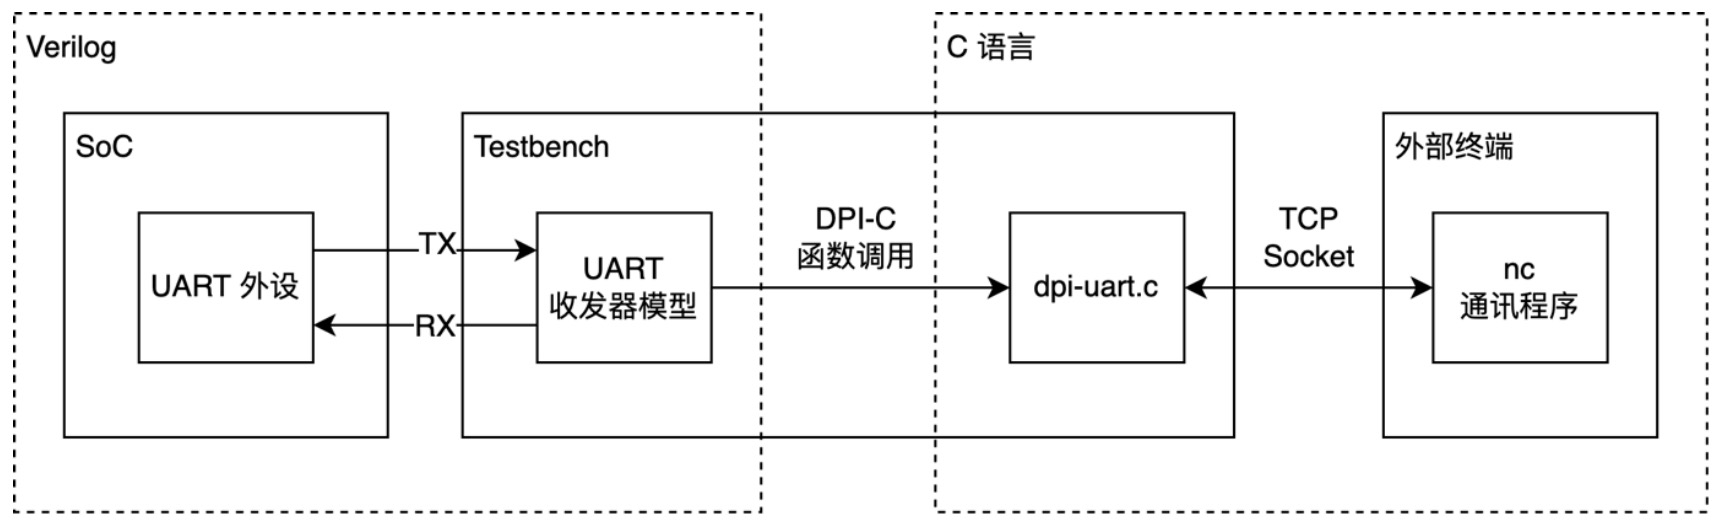
\includegraphics[width=0.75\linewidth]{assets/06/uart-sim.png}
  \caption{UART DPI 仿真模型结构}
  \label{fig:06-uart-sim}
\end{figure}

（2）Ethernet

以太网的仿真与上述串口仿真的实现思路类同，其交互对象为Linux内核提供的TAP接口。TAP接口是Linux内核提供的虚拟网卡接口，允许应用程序模拟网卡收发数据包，从而连通仿真CPU与主机的网络栈，使得仿真CPU能够直接和主机进行网络通，其整体结构如图所示：

\begin{figure}[htbp]
  \centering
  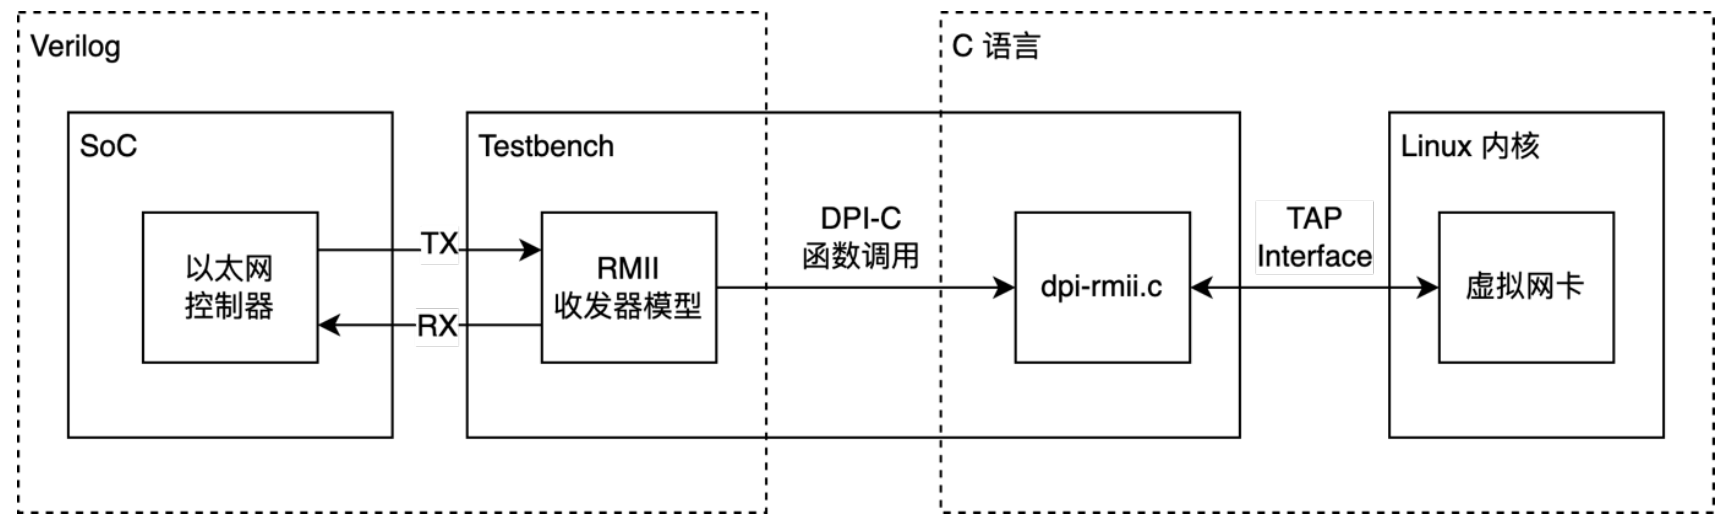
\includegraphics[width=0.75\linewidth]{assets/06/ethernet-sim.png}
  \caption{以太网 DPI 仿真模型结构}
  \label{fig:06-ethernet-sim}
\end{figure}
